\section{Measuring optimal I/O speeds}
\label{sec:optimality}

This section discusses how we compute optimal performance, describes
our cluster environment, and presents measurements of actual disk and
network speeds on our cluster.

\minorsection{Notions of optimality} Optimal efficiency is all
relative, but some notions of optimality may not ever be achievable in
practice.  Since our focus is on hardware optimality, we might look to
the maximum raw hardware speeds for a theoretical notion of
optimality.  However, since the actual hardware performance delivered
by the filesystem and operating system is less than this theoretical
maximum, we prefer an empirical approach to determine the baseline
achievable hardware performance.

Even when restricting ourselves to measured performance from the
operating system, it is difficult for real hardware to sustain maximum
throughput over an extended period of time.  A TCP flow, for instance,
is in a constant state of flux, measuring the perceived round trip
times and performing congestion control operations that affect the
rate of data transfer.  Other factors such as switch buffer overflows
during periods of high congestion can also lead to dropped packets,
TCP timeouts, or even catastrophic network collapse~\cite{incast}.

Because there is a natural performance variability to real hardware,
we first measured both the maximum and average attainable speeds for
our network and disk using basic measurement tools (\texttt{dd} and
\texttt{iperf}), made sure that we were getting the most out of those
resources, and used the average speed numbers in our model of
optimality.  So in that sense, our notion of optimality should be
approachable for an efficient program, although the inevitable
overhead of a useful application that manages many threads and
processes across machines probably means that even this ''average''
notion of optimality is probably not fully possible for any useful
application.

In cases where we do not have the hardware available to do our own
measurements, specifically for the published benchmarks in
Section~\ref{sec:benchmarks}, we make educated and conservative
estimates of the disk and network speeds and specify these estimates
to the reader.  The next two subsections describe these measurements and
how they affect the model.

Finally, our notion of optimality also depends on which operations are
being performed at the hardware level that are necessary to meet the
goals of the application.  When Hadoop writes out intermediate map
output data even in a situation where the failure case is uncommon, we
include that extra operation in our model calculation.

\minorsection{Cluster environment} Our measurements were taken on
CMU's OpenCirrus cluster.  Each node is configured with 2 quad-core
Intel Xeon E5430 processors, 4 1TB Seagate Barracuda ES.2 SATA drives,
and 16 GB of RAM.  The network infrastructure is 1 Gigabit Ethernet
with the greater cluster spread across 4 48-port Force10 switches and
1 24-port Arista 7124S head-end switch.  The kernel's default TCP
implementation is used, which was TCP Reno configured to use 1500 byte
packets. All machines run the Linux 2.6.24 Xen kernel, but none of our
experiments were run in virtual machines -- they were all run directly
on domain zero.

\minorsection{Disk performance} For sufficiently large sequential disk
transfers, seek times have a negligible affect on performance; raw
disk I/O throughput approaches the maximum transfer rate of the disk.
Our newer disks are capable of speeds up to 108 MB/s, while our disk
drives that are 3 to 5 years old typically can transfer around 65
MB/s.  However, these maximum transfer speeds also depend on the
location of the data on disk -- the outer zones of a disk pack more
sectors per track, allowing for faster data transfers than the zones
that are closer to the spindle.

Older, well-used filesystems may also be affected by fragmentation,
which can interrupt sequential transfers with otherwise unnecessary
disk seeks.  These issues can be solved by wiping and repartitioning
the disks.  Therefore, we avoid dealing with fragmentation in our
model.

Disks are also limited by filesystem performance.
Figure~\ref{fig:disk_measurements} presents measurements of read and
write speeds for a few representative transfer sizes on our Seagate
Barracuda drives.  We compare measurements of the raw partition, by
writing directly to the device, to measurements taken with newly-built
\texttt{ext3} and \texttt{xfs} filesystems on the first (outermost)
zone of the disk.  These measurements were made using the \texttt{dd}
utility with 64~MB block sizes and averaged over 10 runs.  The write
experiments use data from \texttt{/dev/zero}, the read experiments
immediately discard their data into \texttt{/dev/null}, and all
experiments sync and free the linux buffer cache before every run.
The potential speedup effects of the disk's write buffer are
negligible because the buffer size is insignificant in comparison to
the data transfer size.

{
\renewcommand{\baselinestretch}{1.0}
\begin{figure}[t]
\begin{center}

%\resizebox{\columnwidth}{!} {
%   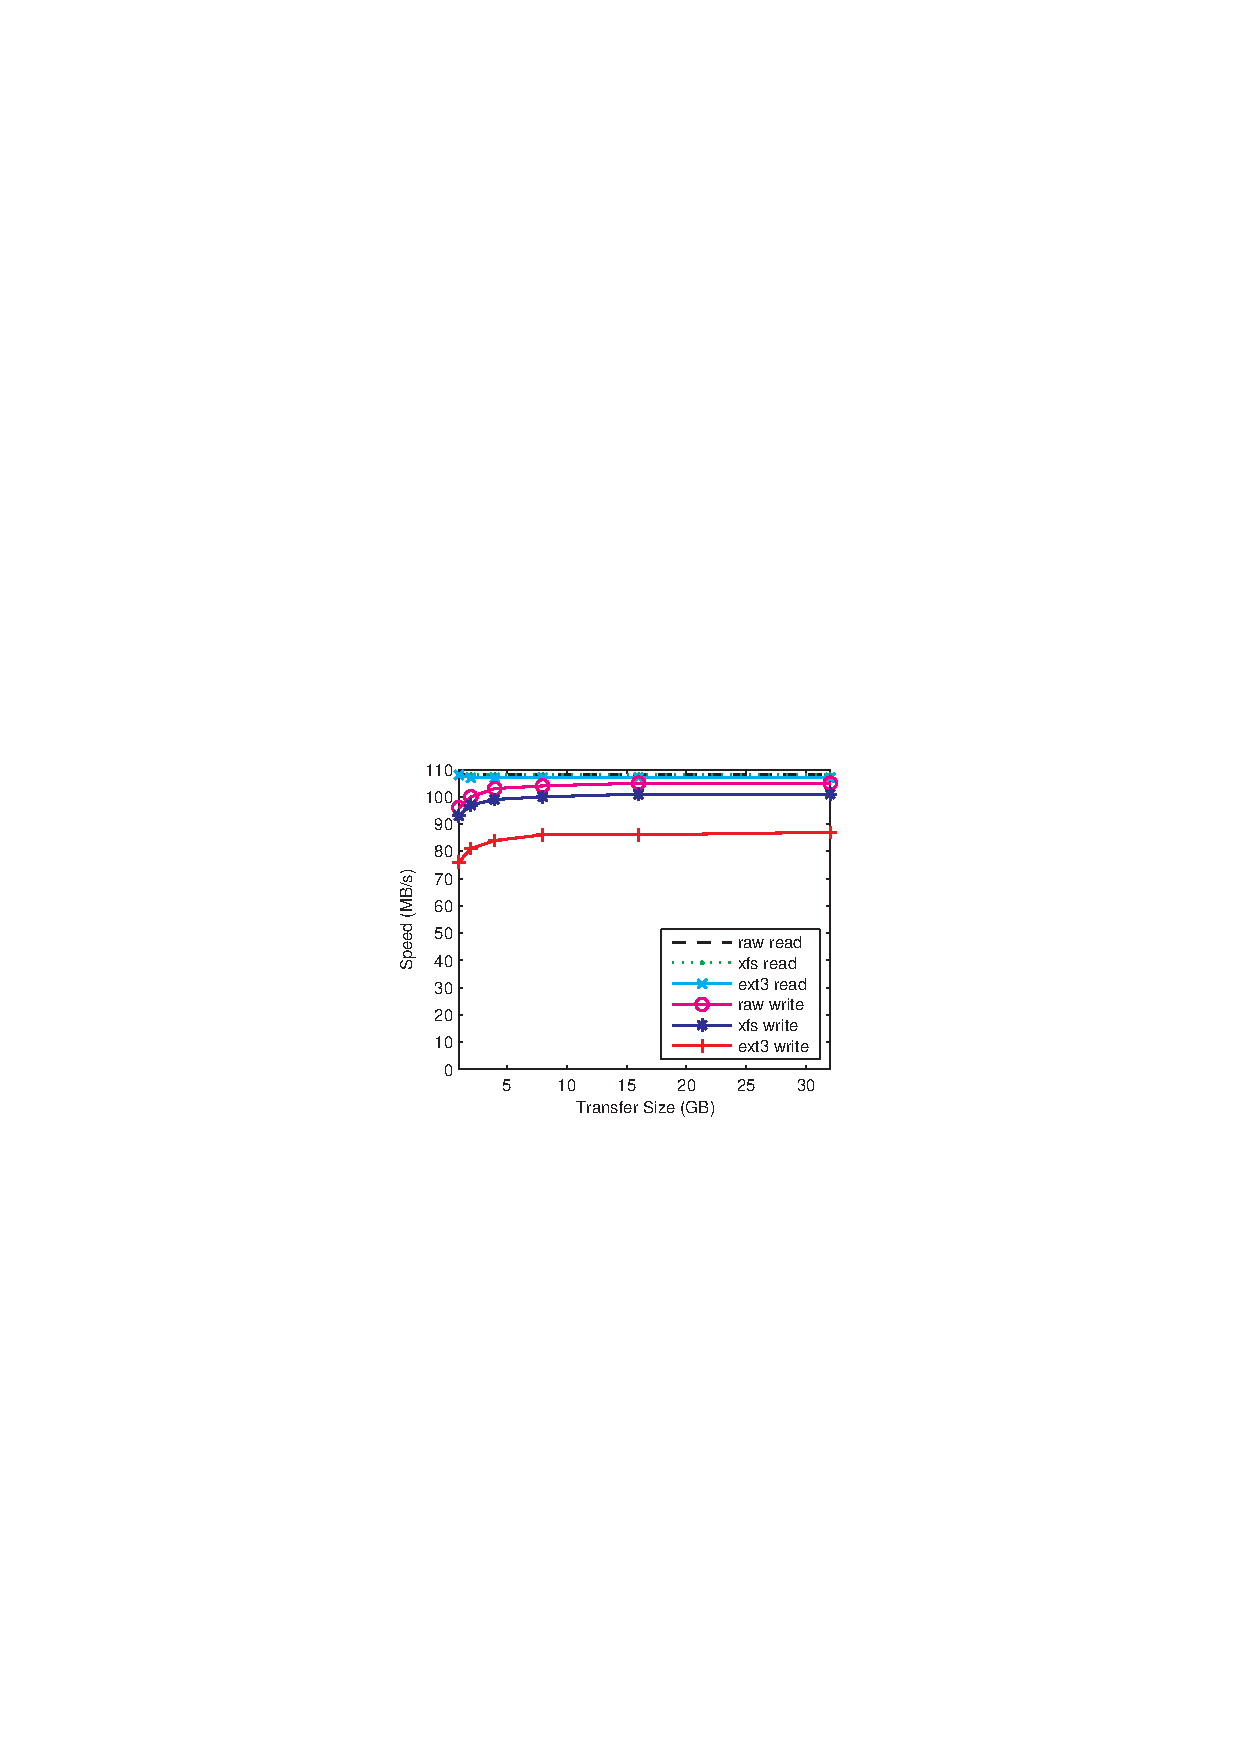
\includegraphics[height=2.5in]{fig_disk_measurements.pdf}
   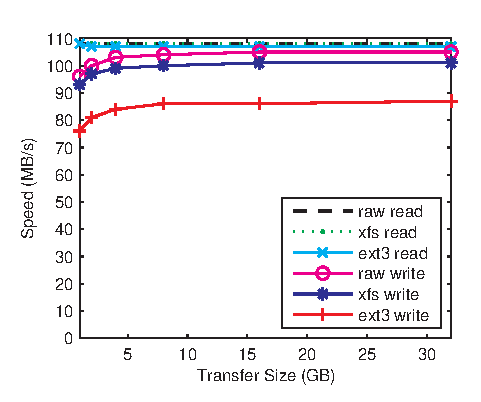
\includegraphics[height=2.5in]{fig_disk_measurements.eps}
%  }

\end{center}
\minicaption{Disk read and write measurements for a Seagate Barracuda drive}
{While read performance is consistently high across all systems,
  writes are slower, and \texttt{ext3} writes in particular are around
  20\% slower than raw device writes.}  

\label{fig:disk_measurements}
\end{figure}
}



Our results show that Gigabyte-sized writes can be up to 32 MB/s
slower than reads.  On the raw partition, this difference is smaller
and becomes insignificant as the transfer size increases.  However, on
ext3 and to a lesser extent on xfs, these differences become smaller
but still persist for larger transfer sizes.

The fact that writes take longer than reads is not a surprise, since
disks are more careful about positioning over a sector before
modifying its physical state.  \texttt{xfs} and \texttt{ext3} also
maintain metadata and a system journal for improved data consistency,
which leads to some natural overhead.  The most likely reason for
\texttt{ext3}'s slower writes is its block allocator, which only
allocates one 4 KB block at a time, and contrasts with \texttt{xfs}'s
variable-length extent-based allocator.  To address some of these
shortcomings, the \texttt{ext4} filesystem improves the design and
performance of \texttt{ext3} by adding, among other things, the
capability for multi-block allocation in a single call~\cite{Kumar08}.

Using the above results, we settled on XFS for use in all our
subsequent experiments to get the fastest speeds, and a file size of
4~GB per node to both achieve fast disk speeds and be able to keep all
our intermediate data in memory. However, since limiting a disk to
only the first zone in practice would be impractical, we also measured
read and write speeds for an XFS filesystem on a partition that
included the entire disk.  After initializing a new XFS filesystem, we
performed the same measurements as before.  Read speeds for 4~GB-sized
files consistently remained unchanged at 108 MB/s.  However, we
noticed more fluctuations in XFS write speeds than before, within a
range of 92-102 MB/s with an average of 97 MB/s over 10 runs.
Therefore, we use 108 MB/s as the optimal read speed and 97 MB/s as
the optimal write speed in our model when calculating optimal times
for our experiments.

\minorsection{Network performance} The actual networks used in many
large data-intensive computing clusters are generally 1 or 10 Gigabit
Ethernet (GBE), due in large part to the commodity pricing of Ethernet
switches and the wide acceptance of TCP/IP.  Other specialized
networks such as Infiniband and FibreChannel are also alternatives.
These networks feature a hierarchy of switches and generally trunk and
over-provision internal links such that a node's link capacity to its
immediate switch is the bottleneck of any parallel data
transfer~\cite{Grider06, Leiserson85}.

Using \texttt{iperf} with the maximum kernel-allowed 256~KB TCP
window size, we tested the network bandwidth between two machines on
the same switch.  Between two machines, we were able to sustain around
900 Mbps, or 112.5 MB/s over a few long-running flows.  TCP/Ethernet
has a natural overhead which makes these speeds fairly competitive for
our 1 GBE links.  Unfortunately, those speeds could not be sustained
over more active connections.  When we measured the aggregate speeds
through any one link in a 5 node all-to-all network transfer, we
achieved around 830 Mbps, or about 104 MB/s.  Based on these
measurements, it appears that our model for network performance at
scale may not be as simple as a single speed.  For now, though, we use
a conservative 110 MB/s of network throughput in the model when
computing optimal performance.
